% !TEX root = ../Appunti_Fisica_2.tex

\newgeometry{
    a4paper,
    top=24mm,
    bottom=28mm,
    left=39mm,
    right=39mm,
    heightrounded
}
\partpage{Elettrostatica}
\restoregeometry

\chapter{Forza elettrostatica e Campo elettrostatico}

Un' \emph{interazione} fondamentale, che gioca un ruolo essenziale nella costruzione della materia, è quella elettromagnetica. Un aspetto particolare dell'interazione elettromagnetica è la \emph{forza elettrica} \mkeyword{forza elettrica}: le sue proprietà costituiscono l'argomento dei primi capitoli di questi appunti. \\

La formulazione precisa della legge della forza elettrica è dovuta a Coulomb, il quale eseguì nel 1785 una serie di misure sistematiche per stabilire la dipendenza della forza tra due cariche dai valori $q_1$ e $q_2$ di queste e dalla loro distanza $r$.\\ 
\mkeyword{Legge di Coulomb} Coulomb stabilì che due \emph{cariche puntiformi} $q_1$ e $q_2$, poste a distanza $r$, interagiscono con una forza $\mathbf{F}$, diretta secondo la loro congiungente, di modulo 

\begin{equation}
    F = k \frac{q_1 \ q_2}{r^2}
\end{equation}

Quindi la forza elettrostatica è direttamente proporzionale al prodotto delle cariche elettriche e inversamente proporzionale al quadrato della loro distanza. \\

L'unità di misura della carica elettrica è il coulomb, simbolo C \mkeyword{coulomb (C)}, che è pari alla carica trasportata in 1 secondo da una corrente di 1A.\\

Il valore di k nel vuoto risulta 

\begin{equation*}
    k = 8.99 \cdot 10^9 \ Nm^2/C^2 \approx 9 \cdot 10^9 \ Nm^2/C^2
\end{equation*}

Per ragioni pratiche è conveniente scrivere k come:

\begin{equation*}
    k = \frac{1}{4 \pi \varepsilon_0}
\end{equation*}

dove la costante $\varepsilon_0$ è nota come costante dielettrica \mkeyword{costante dielettrica} e ha il valore 

\begin{equation*}
    \varepsilon_0 = 8.85 \cdot 10^{-12} \ \frac{C^2}{Nm^2}
\end{equation*}

A seguito dell'ultima ridefinizione del Sistema Internazionale, il valore della carica elementare \mkeyword{carica elementare} espresso in Coulomb è fissato pari a 

\begin{equation*}
    e = 1.602 \cdot 10^{-19} C
\end{equation*}

\newpage

Allora considerate due cariche $q$ e $q_0$ possiamo scrivere la forza elettrostatica che la carica $q$ esercita sulla carica $q_0$ come

\begin{tcolorbox}[colback=yellow!10!white, colframe=orange!70!black, boxrule=0.8pt]
\begin{equation}
    \mathbf{F} = \frac{1}{4 \pi \varepsilon_0} \ \frac{q \ q_0}{r^2} \mathbf{u}
\end{equation}
\end{tcolorbox}

Dove $\mathbf{u}$ è il versore del vettore $\mathbf{r}$ che va da $q$ a $q_0$.\\

\section{Campo elettrostatico}

Le forze elettriche agenti su una carica $q_0$ dovute alle cariche circostanti si sommano come vettori: vige cioè il principio di sovrapposizione \mkeyword{principio di sovrapposizione}, pertanto possiamo scrivere. 

\begin{equation*}
    \mathbf{F} = \sum_i \mathbf{F}_i = q_0 \sum_i \frac{1}{4 \pi \varepsilon_0} \ \frac{q_i}{r_i^2} \mathbf{u}_i
\end{equation*}

Si nota così che la forza elettrica risultante esercitata su $q_0$ è proporzionale a $q_0$. \\
Possiamo andare così a definire la grandezza vettoriale 

\begin{tcolorbox}[colback=yellow!10!white, colframe=orange!70!black, boxrule=0.8pt]
\begin{equation}
    \mathbf{E} = \frac{\mathbf{F}}{q_0}
\end{equation}
\end{tcolorbox}

che prende il nome di campo elettrico \mkeyword{campo elettrico}.\\
L'unità di misura del campo elettrico è $N/C$

E quindi dalla legge di Coulomb si ottiene:

\begin{equation}
    \mathbf{E}(x,y,z) = \sum_i \frac{1}{4 \pi \varepsilon_0} \ \frac{q_i}{r_i ^2} \mathbf{u}_i
    \label{eq: campo elettrostatico}
\end{equation}

Il campo elettrostatico in un punto $P$ prodotto da un sistema discreto di cariche è uguale alla somma dei campi elettrostatici prodotti singolarmente dalle cariche. 

\begin{figure} [h]
    \centering
    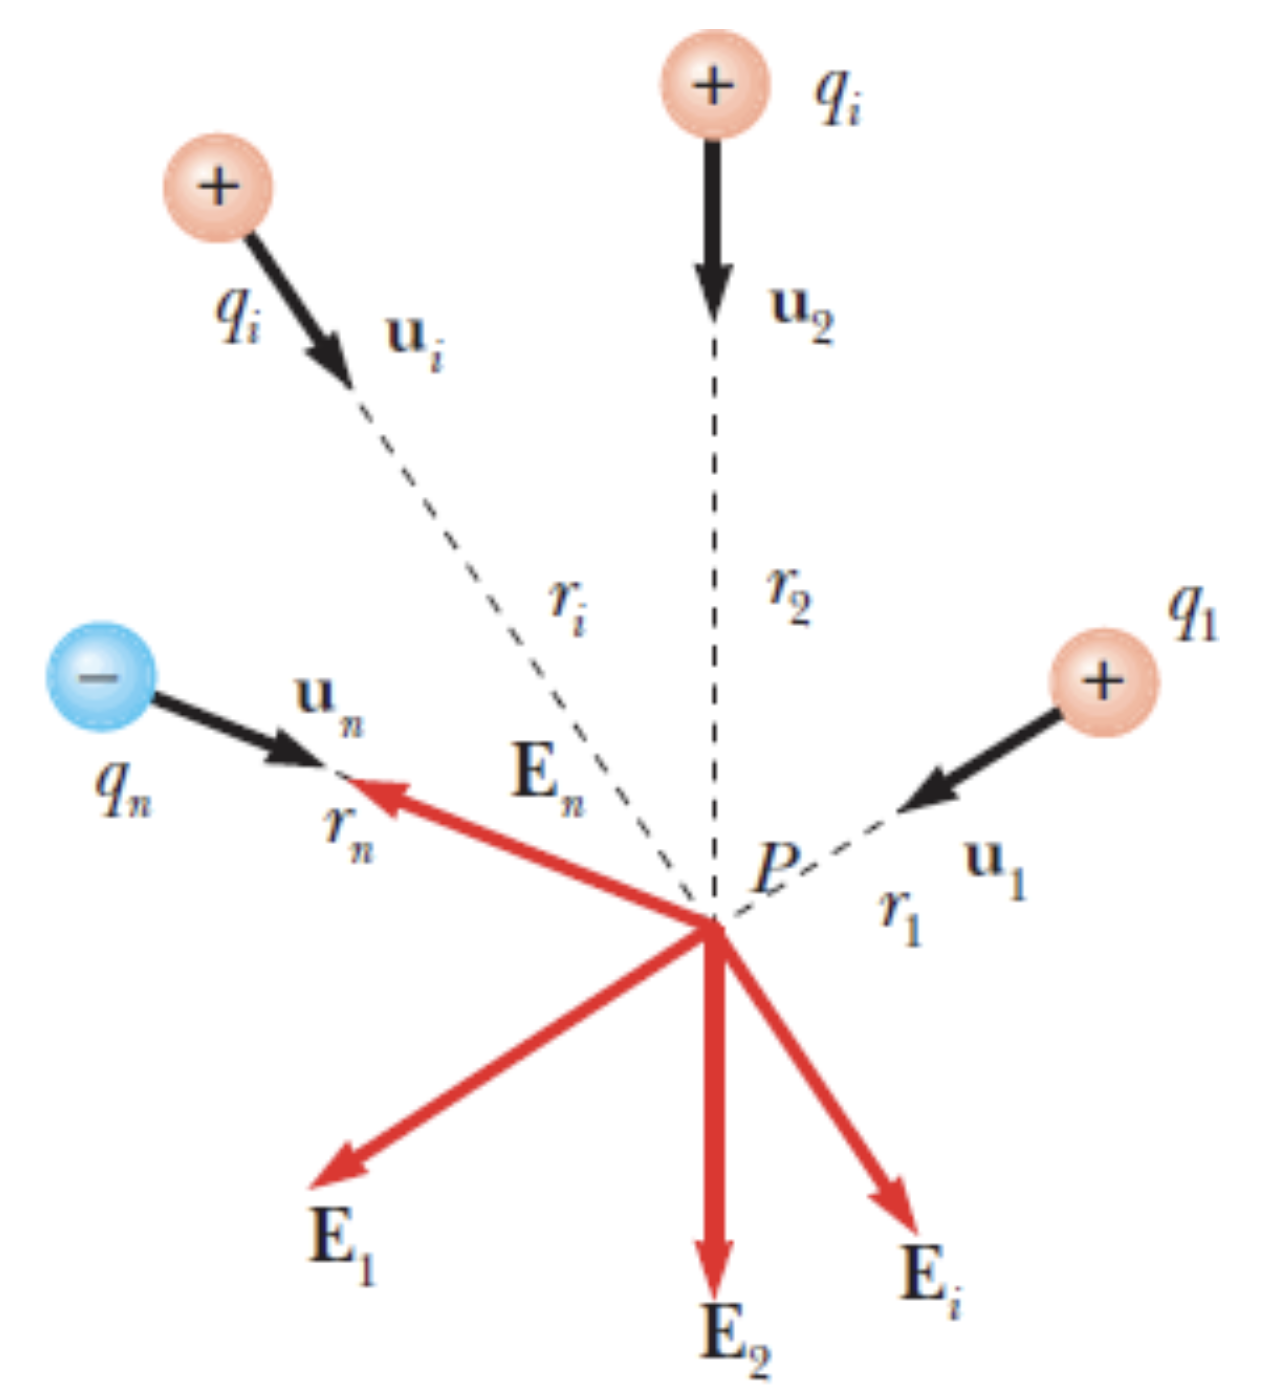
\includegraphics[width=0.4\linewidth]{figure/image1.png}
    \caption{Campo elettrostatico di un sistema discreto di cariche}
    \label{fig:chapter_1_1}
\end{figure}

Le cariche di interesse nei problemi corrispondono a un numero molto grande di cariche elementari, inoltre nella maggior parte dei casi queste non sono concentrate in un unico punto, ma sono distribuite nello spazio con una ben determinata geometria.\\

Supponendo che $\rho (x,y,z)$ sia la densità spaziale di carica, possiamo modificare la \ref{eq: campo elettrostatico} in modo da passare dal caso discreto a quello continuo.

\begin{tcolorbox}[colback=yellow!10!white, colframe=orange!70!black, boxrule=0.8pt]
\begin{equation}
    \mathbf{E}(x,y,z) = \frac{1}{4 \pi \varepsilon_0} \int_V \frac{dq}{r^2} \mathbf{u} =  \frac{1}{4 \pi \varepsilon_0} \int_V \frac{\rho(x,y,z)}{r^2} dV \mathbf{u}
    \label{eq:campo_elettrostatico_continuo}
\end{equation}
\end{tcolorbox}

Lo stesso vale anche per i casi in cui si stia trattando con densità superficiali e lineari di carica. 

\begin{figure} [h]
    \centering
    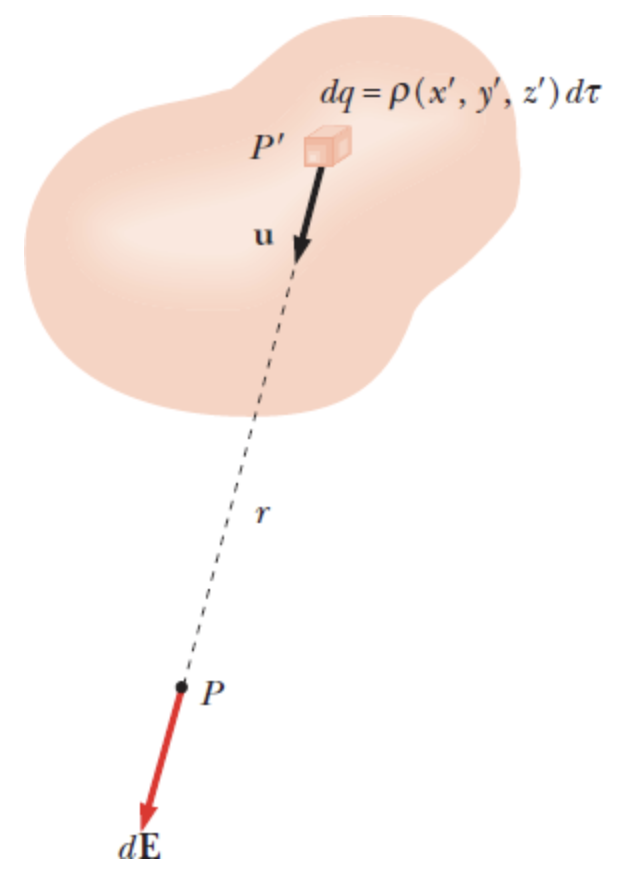
\includegraphics[width=0.4\linewidth]{figure/image3.png}
    \caption{Campo elettrostatico prodotto da un elemento di una distribuzione di carica}
    \label{fig:chapter_1_2}
\end{figure}

\subsection{Linee di forza del campo elettrostatico}

Partendo da una generica posizione e muovendosi per tratti infinitesimi successivi, ciascuno parallelo e concorde al campo elettrostatico in quel dato punto, si ottiene una linea che è detta linea di forza o linea del campo elettrostatico. \mkeyword{linea di forza}\\

Già a questo punto si possono desumere le proprietà delle linee di forza:

\begin{enumerate}
    \item le linee di forza non si incrociano mai, in quanto in ogni punto il campo è definito univocamente e non può avere due direzioni distinte;
    \item le linee di forza hanno origine dalle cariche positive e terminano sulle cariche negative, qualora ci siamo cariche di uno stesso segno le linee di forza si chiudono all'infinito. 
\end{enumerate}
